\documentclass[a4paper,francais]{article}
\usepackage[utf8]{inputenc}
\usepackage[T1]{fontenc}
\usepackage[french]{babel}

\usepackage{subfig}
\usepackage{graphicx}
\graphicspath{{fig/}}
\newcommand{\caserne}{\begin{picture}(0,0) \put(255,100){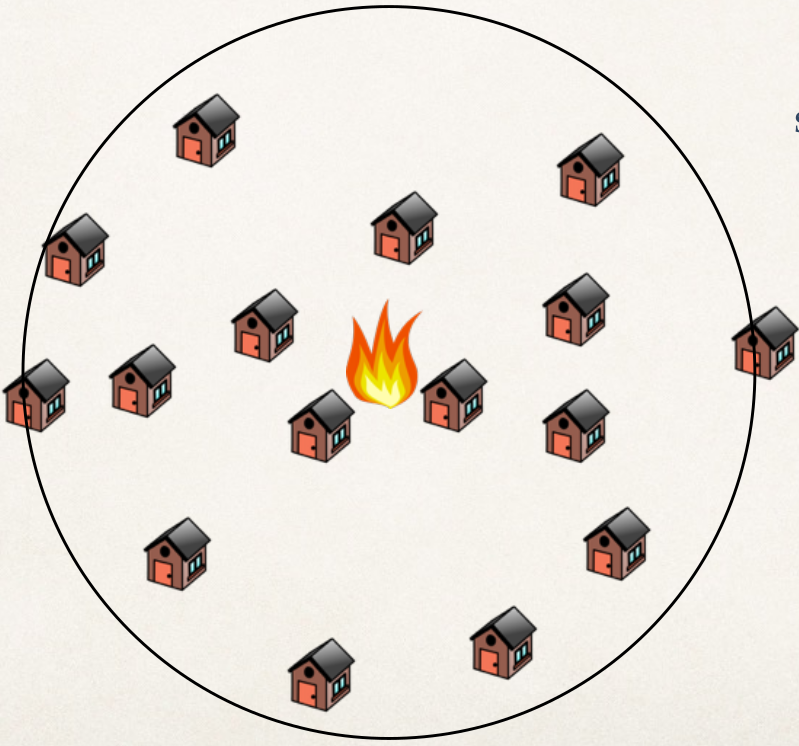
\includegraphics[width=25mm]{caserne}} \end{picture}}

\usepackage{amsmath}
\usepackage{amssymb}
\usepackage{amsthm}
\usepackage{cancel}
\usepackage{enumitem}

\usepackage{hyperref}

\usepackage{cprotect} %verbatim in footnote

\newcommand{\cad}{c.-à-d.}
\newcommand{\Z}{{\ensuremath\mathbb{Z}}}
\newcommand{\N}{{\ensuremath\mathbb{N}}}
\newcommand{\R}{{\ensuremath\mathbb{R}}}
\newtheorem{Theorem}{Theorem}
\newtheorem{Exemple}{Exemple}

%-------- enable or disable correction -----------------------------
\theoremstyle{definition}
\newtheorem{exercice}{Exercice}[section]
\newtheorem*{solution}{Solution}

\usepackage{comment}
\excludecomment{solution}% commenter/décommenter pour afficher/effacer l'impression des solutions


\title{Où placer les pompiers ? \\ \large Résoudre un problème d'optimisation convexe}
\author{Tristan Roussillon}

\begin{document}

\maketitle
\caserne

\section{Introduction}

Nous nous intéressons au problème suivant : étant donné un ensemble $E$ de points dans le plan, 
trouver le plus petit disque contenant $E$. Dit autrement, son centre est le point du plan qui minimise 
la distance maximale avec les points de $E$. C'est un problème simple à comprendre qui a 
toujours une solution unique. Il a des applications variées (localisation optimale, 
apprentissage automatique, vision par ordinateur, informatique graphique, etc.). 
De nombreux algorithmes combinatoires existent pour ce problème, mais nous allons le résoudre
numériquement, à l'aide de la méthode de Frank et Wolfe.

\section{Formulation du problème}

\'Etant donné un ensemble de $n$ points du plan $\{(x_i, y_i)\}_{i = 1, \dots, n}$,
nous considérons le problème d'optimisation sous contrainte suivant :
\[
\text{(P)}
\left\{
\begin{array}{ll}
  \min_{c_x, c_y, r} \ r \ \text{tel que} & \\
  \sqrt{(x_i - c_x)^2 + (y_i - c_y)^2} \leq r & \forall i = 1, \dots, n \\ 
  c_x, c_y, r \in \R \\
\end{array}
\right.
\]

\begin{exercice}
  Donnez une interprétation géométrique des variables $c_x, c_y, r$ et montrez en quoi
  le problème (P) est une formalisation correcte du problème énoncé plus haut.
\end{exercice}

\begin{exercice}
  \`A l'aide du changement de variable $\rho :=c_x^2 + c_y^2 - r^2$, reformulez (P) en un
  problème (P') ayant une fonction objective sous la forme d'un polynôme de degré 2 et
  des contraintes linéaires.
  %sous la forme de combinaisons linéaires des variables inférieures à une constante.
  Piste : mettre au carré, développer l'inégalité, opérer le changement de variable.
  Faites valider par l'enseignant. 
\end{exercice}

\begin{solution}
\[
\text{(P')}
\left\{
\begin{array}{ll}
  \min_{c_x, c_y, \rho} \ c_x^2 + c_y^2 - \rho \ \text{tel que} & \\
  (-2x_i) c_x + (-2y_i) c_y + \rho  \leq -(x_i^2 + y_i^2) & \forall i = 1, \dots, n \\ 
  c_x, c_y, \rho \in \R \\
\end{array}
\right.
\]
\end{solution}

\begin{exercice}
  Calculez le gradient et le hessien de la fonction objective de (P').
  Calculez les trois valeurs propres du hessien\footnote{Vous pouvez
    vérifier avec \url{http://www.arndt-bruenner.de/mathe/scripts/engl_eigenwert2.htm}}.
  Déduisez-en que c'est une matrice semi-définie positive et que la fonction est convexe. 
\end{exercice}

\begin{solution}
  Le hessien de la fonction objective notée $f$ est
  \[
    {\nabla^2f}(c_x,c_y,\rho) =
    \begin{pmatrix}
      2 & 0 & 0 \\
      0 & 2 & 0 \\
      0 & 0 & 0 \\
    \end{pmatrix}
  \]
  Il est constant et noté plus simplement $H$.
  
  Ses valeurs propres sont les valeurs $\lambda(\lambda_1, \lambda_2, \lambda_3)$
  vérifiant $\det{(\lambda I - H)} = 0$. En développant le déterminant, on obtient
  l'égalité $\lambda_3(\lambda_1 - 2)(\lambda_2 - 2) = 0$, ce qui signifie que les
  valeurs propres sont $2, 2$ et $0$, toutes positives, d'où l'on déduit que
  H est semi-définie positive, et par suite, comme le hessien de $f$ l'est partout,
  que $f$ est convexe. 
\end{solution}

\section{Résolution numérique du problème en python}

Vous avez un problème d'optimisation convexe sous contraintes linéaires. Dans cette
section, votre objectif est d'écrire un programme python pour le résoudre à l'aide
de la méthode de Frank et Wolfe
\footnote{Voir aussi \url{https://en.wikipedia.org/wiki/Frank\%E2\%80\%93Wolfe_algorithm}}. 

\begin{exercice}
  \'Ecrivez un script python qui génère aléatoirement un ensemble de 100 points se trouvant
  dans le cercle de centre $(0,0)$ et de rayon $100$. Utilisez un moyen à votre convenance
  pour afficher les points et le cercle solution (matplotlib, svg, etc.)   
\end{exercice}

\begin{exercice}
  \`A l'aide d'un solveur d'optimisation linéaire, écrivez une fonction
  qui minimise une fonction linéaire en $c_x, c_y, \rho$ sous les contraintes de $(P')$.

  Vous pouvez utiliser
  \href{https://docs.scipy.org/doc/scipy-1.3.3/reference/generated/scipy.optimize.linprog.html#scipy.optimize.linprog}{\texttt{linprog}} ou
  \href{https://docs.scipy.org/doc/scipy-1.3.3/reference/generated/scipy.optimize.minimize.html}{\texttt{minimize}}.
  Le plus délicat est de décrire correctement les données nécessaires au solveur.
  Vous aurez aussi besoin de
  \href{https://docs.scipy.org/doc/numpy/reference/routines.array-creation.html}{créer} et
  \href{https://docs.scipy.org/doc/numpy/reference/routines.array-manipulation.html}{manipuler} des
  tableaux
  \href{https://numpy.org/doc/stable/contents.html#numpy-docs-mainpage}{\texttt{NumPy}}. 
\end{exercice}

\begin{exercice}
  \'Ecrivez une fonction qui résoud (P') selon la méthode de Frank et Wolfe.
  \`A chaque étape, vous devez utiliser votre fonction précédente comme routine. 
  Pour l'initialisation, vous pouvez fixer $(c_x, c_y)$ à $(0,0)$ et $r$ à la
  distance maximale entre l'origine et les points de l'ensemble, ce qui assure
  la couverture de tous les points de l'ensemble.
\end{exercice}

\end{document}


